\section{Theory}

Given a polygon $\mathcal P$ and a guard $p(x, y) \in \mathcal P$, we are interested in defining the gradient for computing the best change in the position of $p$.

We will compute the gradient by fixing the $x$-coordinate of $p$ and varying its $y$-coordinate. The reason behind this choice is the fact that the computation of the gradient remains the same regardless of the rotation applied to the plane.

We define $f(p)$ as the area seen by a guard $p$, and $f'_i(p)$ the local change in the area seen by guard $p$ around reflex vertex $i$, as given by the derivative of $f$. The total (global) change in the area seen by $p$ can be thus summed up to $f'(p) = \sum_i f'_i(p)$.

Let $\bigtriangledown f = (\frac{\partial f}{\partial x}, \frac{\partial f}{\partial y})$ be the gradient of guard $p(x, y)$ given the change in position of $p$ on the $y$-axis. That is, the direction of the greatest increase of $f$. 

% We consider the case where there is only a positive change in the $y$ position of $p$. The case with a negative coordinate change would be analogous.

Let $g$ be a boundary line of $\mathcal P$, $r$ a reflex vertex of $\mathcal P$ and $p$ a guard whose position requires optimisation with respect to $r$. Let $\overline{pr} = \alpha$. Additionally, let $d$ be the maximum point on $g$ that $p$ can see behind $r$. The distance between $r$ and $d$ is considered as $|\overline{rd}| = \beta$. 

Let $\partial x$ be the extremely small change in the position of $p$ to a new position $p'$. $p'$ can see up to a new maximum point $d'$ around $r$ on $g$. Let the distance between $d$ and $d'$ be $|\overline{dd'}| = L$. As such, $\triangle rdd'$ becomes the increase in the visibility area of $p$ when it moves to position $p'$. 

% Let $a''$ be the projection of $p'$ on $p''r$, and $a$ the projection of $a''$ on the line $pr$ such that the distance from $a$ to $r$ is $|\overline{ar}| = \alpha$. Take the distance between $p$ and $p'$ to be $x$. Since $a''$ is the projection of $p'$ on $pr$, then $|\overline{pp'}| = |\overline{aa''}| = x$.





% \subsection{Canonical Case}
Consider the geometrical construction in Figure \ref{fig:gradient}. The construction was created for ease of computation, and the general case can be translated and rotated to this case.

In this canonical case we will consider the situation where the gradient is normalised as $||\bigtriangledown f|| = 1$. 

We are now interested in computing the distances $\partial x$, and $L$ such that we can compute the increase in the area seen by $p$ and thus the gradient $\bigtriangledown f$. Computing $\bigtriangledown f$ is thus equivalent to computing the change in the area of triangle $\triangle rdd'$.
% We are now interested in computing the distances $|\overline{df}|, |\overline{aa'}|, |\overline{pp''}|, L$ such that we can compute the increase in the area seen by $p$ and thus the gradient $\bigtriangledown f$. The two triangle areas that need to be computed in order to do so are $A_{\triangle rdd'}$ and $A_{\triangle rdd''}$.

Given that triangles $\triangle rpp'$ and $\triangle rdd'$ are square triangle, we can compute their areas as follows:

$$\text{Area}_{\triangle rpp'} = \frac{\alpha \partial x}{2}$$

$$\text{Area}_{\triangle rdd'} = \frac{\beta L}{2}$$

Given that $\overline{pp'}$ is parallel to $g$, we can use the Intercept Theorem in triangles $\triangle rpp'$ and $\triangle rdd'$ to compute length $L$: $$\frac{||\overline{pp'}||}{||\overline{dd'}||} = \frac \alpha \beta \iff \frac{\partial x}{L} = \frac \alpha \beta \Rightarrow L = \frac{\beta \partial x}{\alpha}.$$

% we can compute the length $L$: $$\frac{\text{Area}_{\triangle rdd'}}{\text{Area}_{\triangle rpp'}} = \frac{\frac{\beta L}{2}}{\frac{\alpha \partial x}{2}} = \frac{\beta L}{\alpha \partial x} \Rightarrow L = \frac{\partial x \beta}{\alpha}.$$

We are now interested in how areas $\text{Area}_{\triangle rpp'}$ and $\text{Area}_{\triangle rdd'}$ change depending on how $\alpha$ and $\beta$ are varied. That is, $\frac{\text{Area}_{\triangle rdd'}}{\text{Area}_{\triangle rpp'}}$ as a function of $\alpha$ and $\beta$: 

$$\frac{\text{Area}_{\triangle rpp'}}{\text{Area}_{\triangle rdd'}} = \frac{\frac{\alpha \partial x}{2}}{\frac{\beta L}{2}} = \frac{\alpha \partial x}{\beta L} = \frac{\alpha \alpha}{\beta \beta} = {(\frac \alpha \beta)}^2 \Rightarrow \text{Area}_{\triangle rdd'} = {(\frac \beta \alpha)}^2 \frac{\alpha \partial x}{2} = \frac{\beta^2 \partial x}{2\alpha}.$$
% $$\frac{\partial f}{\partial x} = \frac{\text{Area}_{\triangle rdd'}}{\partial x}$$

Thus, the change in the visibility area $\text{Area}_{\triangle rdd'}$ of $p$ given the small change $\partial x$ in the position of $p$ is $$\bigtriangledown f = \frac{\partial f}{\partial x} = \frac{\text{Area}_{\triangle rdd'}}{\partial x} = \frac{\beta^2}{2\alpha}.$$

% Given that $pp''$ is parallel to $g$, we can use the Intercept Theorem to compute the lengths of the segments as follows:

% \begin{itemize}
%     \item in $\triangle raa'$, $\triangle rpp'$, with $aa' || pp'$: $$\frac{|\overline{pp'}|}{|\overline{dd'}|} = \frac{|\overline{pr}|}{|\overline{rd}|} \iff \frac{x}{|\overline{dd'}|} = \frac{1}{\beta} \Rightarrow |\overline{dd'}| = x\beta$$
    
%     $$\frac{|\overline{aa'}|}{|\overline{pp'}|} = \frac{\alpha}{1} = \frac{|\overline{aa'}|}{x} \Rightarrow |\overline{aa'}| = x\alpha$$

%     \item in $\triangle rpp''$, $\triangle raa''$, with $pp'' || aa''$: $$\frac{|\overline{aa''}|}{pp''} = \frac{|\overline{ar}|}{|\overline{pr}|} \iff \frac{x}{|\overline{pp''}|} = \frac{\alpha}{1} \Rightarrow |\overline{pp''}| = \frac{x}{\alpha}$$
    
%     \item in $\triangle rpp''$, $\triangle rdd''$, with $pp'' || dd''$: $$\frac{|\overline{pp''}|}{|\overline{dd''}|} = \frac{|\overline{pr}|}{|\overline{rd}|} \iff \frac{\frac{x}{\alpha}}{L} = \frac{1}{\beta} \Rightarrow L = \frac{x\beta}{\alpha}$$
% \end{itemize}

% Now the area of the square triangle $\triangle rdd''$ corresponding to the gradient $\bigtriangledown f$ can be computed as: $$\bigtriangledown f = \frac{|\overline{rd}||\overline{de}|}{2} = \frac{\beta L}{2} = \frac{\beta \frac{x\beta}{\alpha}}{2} = \frac{\beta^2x}{2\alpha}, ||x|| = 1$$

\begin{figure}[h!]
    \centering
    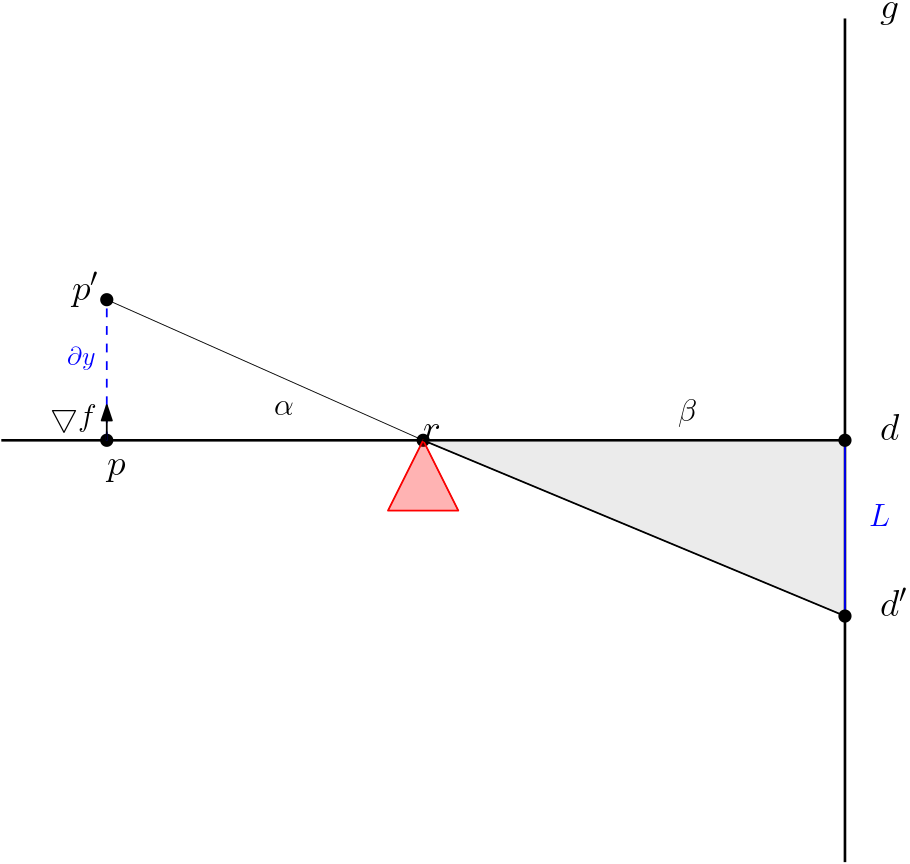
\includegraphics[width = 0.6\textwidth]{gradient2.png}
    \caption{Canonical Gradient Construction.}
    \label{fig:gradient}
\end{figure}


% \subsection{General Case}



% - we will only look at one coordinate (vary $y$), since varying $x$ is symmetrical, but rotated $90^\circ$

% - we will first look at a canonical situation $||\bigtriangledown f|| = 1, \alpha = \beta = 1$

% Let:

% - $f(p)$ - area seen by guard $p$

% - $f'_i(p)$ - the change in the area seen locally by guard $p$, as given by its derivative

% - $f'(p) = \sum_i f'_i(p)$ - the change in the area seen globally by guard $p$

% - $\bigtriangledown f = (\frac{\partial f}{\partial x}, \frac{\partial f}{\partial y})$ - the direction of the greatest increase of $f$

% - $r$ - reflex vertex

% - $p$ - guard whose position needs to be optimised

% - $|\overline{pr}| = 1$

% - $p', p''$ - the new positions of the guard where the $y$-coord is varied

    % - $|\overline{pp'}| = |\overline{aa''}| = x$

% - $\overline{ar} = \alpha, a \in \overline{pr}$ - additional guard construction

% - $\triangle rde$ - area seen by $p$

    % - $\triangle rdf$ - area seen by $p'$

% - $|\overline{rd}| = \beta$ - distance between reflex vertex and polygon boundary

% - $|\overline{de}| = L$

% Using the Intercept Theorem:

% - in $\triangle ra'a$, $\triangle rp'p$: $\frac{|\overline{pp'}|}{|\overline{df}|} = \frac{|\overline{pr}|}{|\overline{rd}|} = \frac{x}{|\overline{df}|} = \frac{1}{\beta} \Rightarrow |\overline{df}| = x\beta$

% - in $\triangle pp'r$, $\triangle aa'r$: $\frac{|\overline{aa'}|}{|\overline{pp'}|} = \frac{\alpha}{1} = \frac{|\overline{aa'}|}{x} \Rightarrow |\overline{aa'}| = x\alpha$

% - in $\triangle pp''r$, $\triangle aa''r$: $\frac{|\overline{aa''}|}{pp''} = \frac{|\overline{ar}|}{|\overline{pr}|} = \frac{x}{|\overline{pp''}|} = \frac{\alpha}{1} \Rightarrow |\overline{pp''}| = \frac{x}{\alpha}$

% - in $\triangle pp''r$, $\triangle rde$: $\frac{|\overline{pp''}|}{|\overline{de}|} = \frac{|\overline{pr}|}{|\overline{rd}|} = \frac{\frac{x}{\alpha}}{L} = \frac{1}{\beta} \Rightarrow L = \frac{x\beta}{\alpha}$

% Computing the area of the square triangle $\triangle rde$:

% - $A = \frac{|\overline{rd}||\overline{de}|}{2} = \frac{\beta L}{2} = \frac{\beta \frac{x\beta}{\alpha}}{2} = \frac{\beta^2x}{2\alpha}$